\documentclass[12pt,a4paper,oneside]{article}
\usepackage[utf8]{inputenc}
\usepackage[francais]{babel}
\usepackage[T1]{fontenc}
\usepackage{mathpazo}
\usepackage[left=3cm,right=2cm,top=2cm,bottom=3cm]{geometry}
\usepackage{graphicx, color, hyperref}
\usepackage{eurosym}


\author{Gildas T. N., Guillaume Z., Jacky M., Sébastien H., Stéphane M.}
\title{\textbf{Résumé de thèse \\ \vspace{0.5cm} \normalsize \og Analyse Sémantique d'un Corpus Exhaustif de Décisions Jurisprudentielles pour l'Élaboration d'un Modèle Prédictif du Risque Judiciaire \fg{} }}

\date{LGI2P(EMA) \& CHROME(UNIMES)}

\begin{document}
\nocite{}

\maketitle

\section{Plus court}

La thèse vise à répondre aux difficultés rencontrées par les juriste lors l'analyse manuelle: le volume énorme des décisions (plus de 2 millions prononcées chaque année), la complexité de la justice, l'incompréhensibilité du langage. Il est principalement de proposer des approches d'extraction automatique d'information à partir d'un corpus de décisions de justice pour l'enrichissement d'une base de connaissances. Nous nous intéressons particulièrement aux références de l'affaire, les quanta demandés et accordés, et les facteurs expliquant les décisions, le type d'affaire. La base de connaissances servira à automatiser différents services et analyses comme l'exploration de la jurisprudence, l'analyse de cas similaires, le conseil juridique automatique, la prédiction de décisions de justice.

\section{Plus long}

% Objectif de la thèse

Cette thèse porte sur la structuration de corpus jurisprudentiels par extraction d'information dans des décisions judiciaires. Une décision est un document rédigé par une juridiction, au terme d'une affaire, afin de récapituler les références, les faits, la procédure, les demandes, les solutions décidées par les juges ainsi que leur motivation. Les décisions étant des textes non structurés, le projet a pour objectif de développer des approches d'analyse sémantique à l'aide de techniques de trainement automatique du langage naturel et d'analyse textuel.
%
 
% motivation
L'importance de ce problème tient au fait qu'un corpus jurisprudentiel représente la manière dont les tribunaux interprètent le droit et les lois pour résoudre un problème juridique donné i.e. un type de contentieux. La compréhension de ce corpus est donc un élément incontournable dans le travail des juristes et autre acteur du droit. 

D'une part, pour conseiller ou défendre leurs clients, les avocat doivent se  référer aux décisions passées similaires à leur affaire en cour pour comprendre ce qui motive généralement les juges dans leur prise de décision, afin d'anticiper le risque de leur client. Ces connaissances permettraient par exemple à une personne physique ou morale d'aller vers une négociation ou un procès avec son adversaire. 

D'autre part, l'analyse empirique de corpus jurisprudentiel est généralement réalisée par des chercheurs en droit afin de comprendre comment sont traités certaines types de contentieux. Ce cas est particulièrement intéressant pour nous car contrairement aux avocats qui pourraient se contenter d'une, de deux ou moins d'une dizaine de décisions comme références, les chercheurs ont besoin de traiter un maximum de  cas. Réalisée manuellement, ces travaux de recherche mobilisent généralement de nombreux chercheurs sur plusieurs mois qui ne pourront au final qu'analyser un échantillon faiblement représentatif. 

L'analyse des décisions est difficile à cause de plusieurs facteurs notamment en France, notre contexte d'étude.

Premièrement, l'analyse manuelle d'un corpus exhaustif est quasi impossible au vue de l'énorme volume de décisions à traiter; plus de 2 millions de décisions sont prononcées par an. 

Par ailleurs,  l'accès à une collection d'intérêt est difficile car  les décisions restent généralement au niveau des tribunaux qui ne les publient pas. Malgré la loi Lemaire du 7 octobre 2016 sur la République numérique, la proportion de décisions accessibles librement reste très faible. Quelques moteurs de recherche juridiques publient des décisions en ligne avec un accès payant pour certains et gratuit pour d'autres; les moteurs payant comprenant la plus grosse quantité de décision. De plus, la recherche de décisions sur ces moteurs reste très basique (date, mots-clés, ...) pour des juristes qui s'intéressent à des critères plus fins comme les normes utilisées, un type de demande, un type d'affaire, ...

D'autre part, l'analyse automatique des décisions pourrait être d'une grande aide pour les non juristes qui ne peuvent pas connaitre les risques de leur actes sans l'aide d'un juriste du fait de la complexité de la justice et de l'incompréhensibilité du langage juridique.
%

% problématiques
Pour répondre à ces problèmes, notre projet vise la structuration automatique d'un corpus jurisprudentiel au sein d'une base de connaissance. Les informations extraites comprennent les références (le lieu, la date, l'identifiant, ...), les demandes des parties et les résultats correspondant des juges, les facteurs expliquant ces résultats, et les circonstances factuelles catégorisant les affaires (divorce, licenciement, trouble de voisinage, ...). 

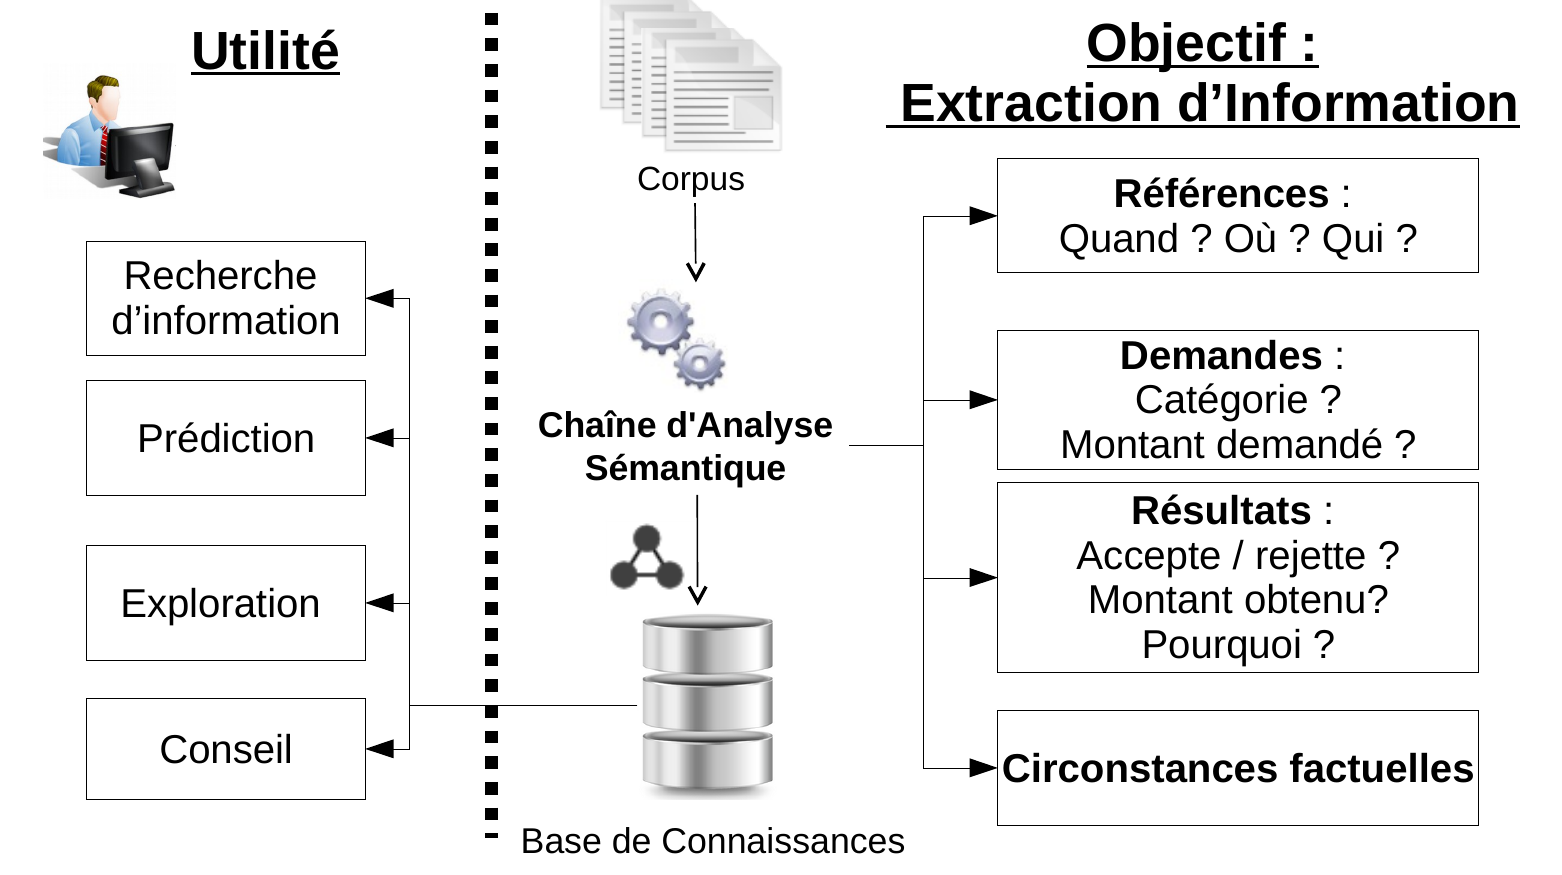
\includegraphics[width=\textwidth]{summary-prj.png}
%


% cas d'utilisation
La base de connaissances ainsi constituée servira à automatiser différents services et analyses comme l'exploration de la jurisprudence, la recherche et l'analyse de cas similaires, le conseil automatique, la prédiction de décisions de justice.

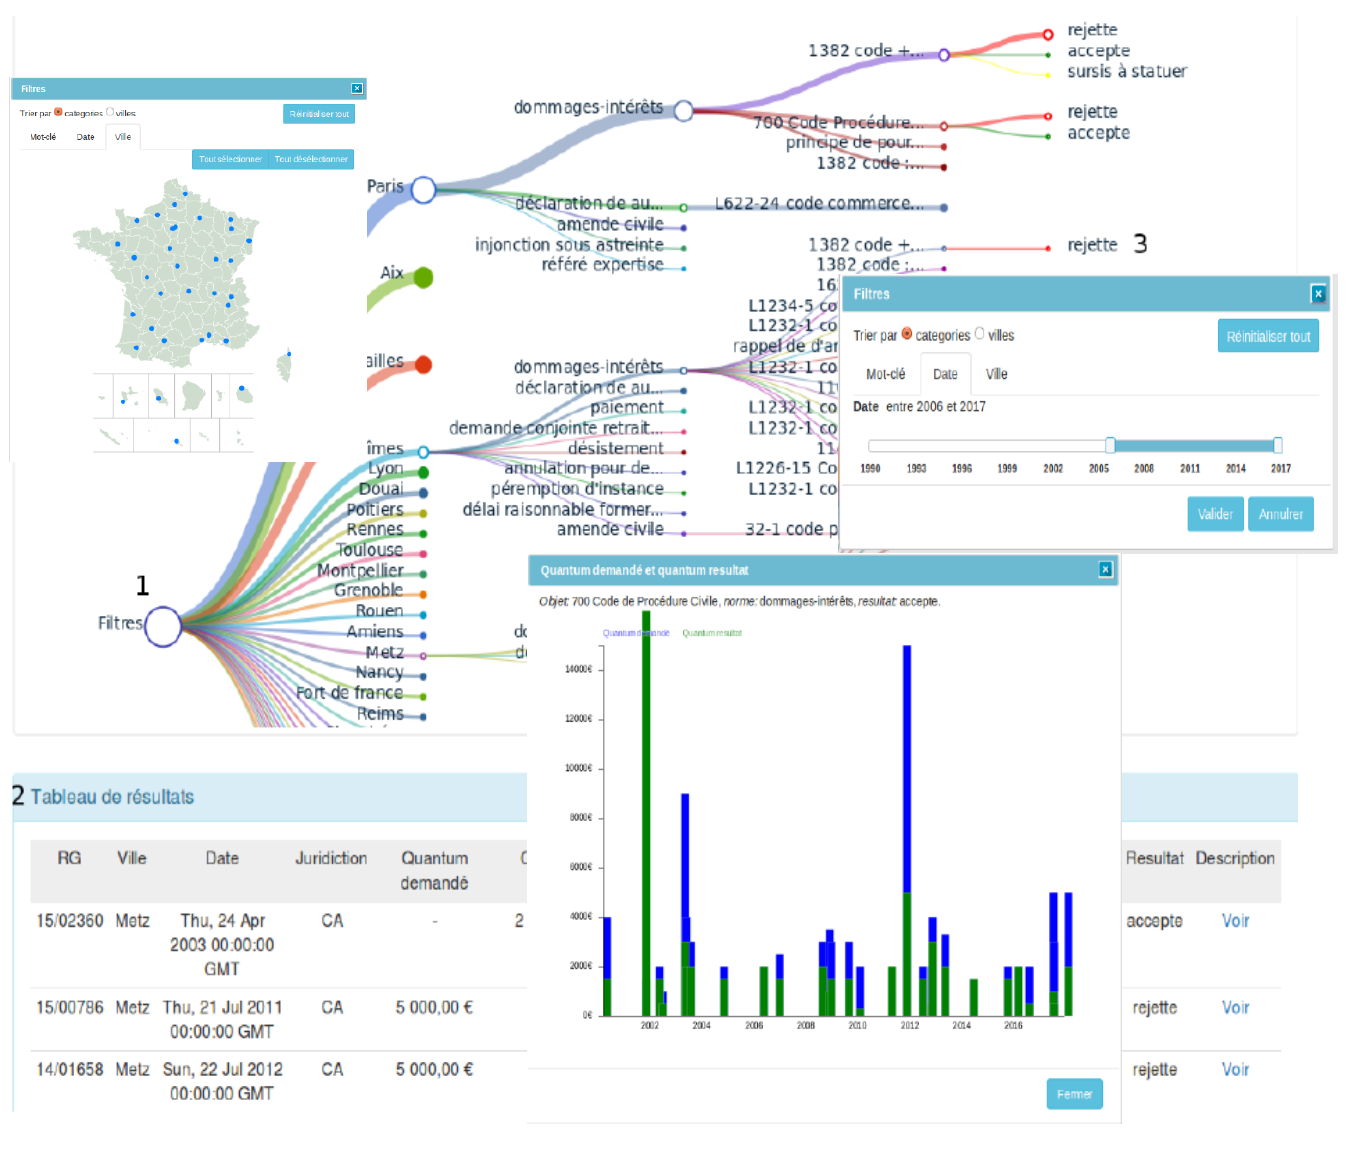
\includegraphics[width=\textwidth]{interface.png}


% contributions actuelles
Pour l'instant, nous avons proposé une approche de sectionnement des documents et d'extraction des entités nommées à l'aide modèles graphiques markoviens. Le sectionnement  permet de séparer les informations de natures différentes et ainsi de mieux organiser l'extraction des informations avec des traitements en fonction des informations et des sections. La reconnaissance d'entités nommées permet quant à elle d'extraire les références, des normes et des sommes d'argent.

Nous avons aussi proposé une approche d'extraction des demandes et résultats associés. L'approche définie une chaine de traitement qui s'adapte en fonction de la catégorie de demande à extraire. Les informations qui nous intéressent pour une demande sont le quantum demandé, le sens du résultat (accepte/rejette), et le quantum accordé.

% difficultés rencontrées
Le projet comporte plusieurs problématiques de traitement de texte intéressantes mais avec de nombreuses difficultés: la traduction de problèmes d'analyse juridique en problèmes d'extraction d'information, la constitution de jeux de données d'évaluation, la particularité des textes, ...

\end{document}
